\documentclass{article}
\usepackage[utf8]{inputenc}
\usepackage{graphicx}
\graphicspath{ {./diagramas/} }

\title{Câmera na Campainha \\ Relatório Final \\ Grupo 14}

\author{Diogo Ribeiro \\\texttt{up201703515} \and Daniel Mendes\\\texttt{up201605245} \and Evan Sá\\\texttt{up201707418} \and Vítor Silva\\\texttt{up201402657}}

\date{Maio 2021}

\begin{document}

\maketitle

\section{Introdução}
\vspace{2mm}
\hspace{0.5cm} O presente relatório tem como objetivo a exposição do desenvolvimento projeto \textbf{Câmara na campainha}, elaborado no âmbito da unidade curricular de Sistemas Embutidos. Este projeto consiste no desenvolvimento de uma campainha inteligente, através da instalação de uma câmara de infravermelhos na porta da residência, um botão que simulará a campainha, e um sensor de movimento cuja função será detetar a presença de pessoas na entrada da casa/apartamento. Após ser detetada alguma atividade na entrada do domicílio, ou ao ser pressionado o botão, a câmara será ativada, gravando e emitindo imagens a tempo real para o \textit{smartphone} do dono da propriedade. Além do utilizador poder realizar um pedido de uma \textit{livestream} após receber notificação de atividade na sua entrada, este também tem a possibilidade de visualizar e apagar todos os vídeos \textit{stop-motion} captadas pela câmara.

\section{Requisitos}
\vspace{2mm}
\hspace{0.5cm} Nesta secção, estão enumerados os requisitos funcionais e não-funcionais essenciais para o correto funcionamento do projeto.

\subsubsection{Requisitos Funcionais}
\vspace{2mm}

\begin{itemize}
    \item O sistema deverá captar imagens gravadas com "stop-motion" através de uma câmara instalada na porta de uma casa/apartamento. Esta câmara será ativada no momento de deteção de movimento pelo sensor ou após um clique no botão que representa a campainha da residência.
    \item Deve haver uma luz vermelha a indicar que a câmara está a gravar.
    \item Após passados 5 minutos de deixar de detetar alguém, o sistema deverá parar.
    \item Posteriormente à ocorrência de um toque na campainha, o utilizador deverá ser notificado do acontecimento no seu smartphone.
    \item A partir do seu smartphone, o utilizador que recebeu notificação poderá requisitar uma stream de vídeo sem "stop-motion".
    \item No smartphone deve também ser possível visualizar os vídeos "stop-motion" gravados pela câmara e apagar os mesmos.
\end{itemize}
\vspace{2mm}

\subsubsection{Requisitos Não Funcionais}
\vspace{2mm}

\begin{itemize}
    \item A deteção de presença de um índividuo na porta pelo sensor deverá ser inferior a 3 segundos.
    \item Após a deteção de presença ou um toque na campainha, o início de gravação deverá ser inferior a 3 segundos.
    \item O pedido de stream de vídeo do smartphone do utilizador deverá ter um atraso inferior a 10 segundos.
    \item A presença física de uma pessoa pelo sensor de movimento terá de ser detetada a uma distância mínima de 50 centímetros.
\end{itemize}

\newpage
\section{Desenvolvimento}
\subsection{Arduino}
\subsection{Raspberry Pi}
\subsection{Android}

\newpage
\section{Diagrama de estados}

    \begin{figure}[h!]
    \centering
    %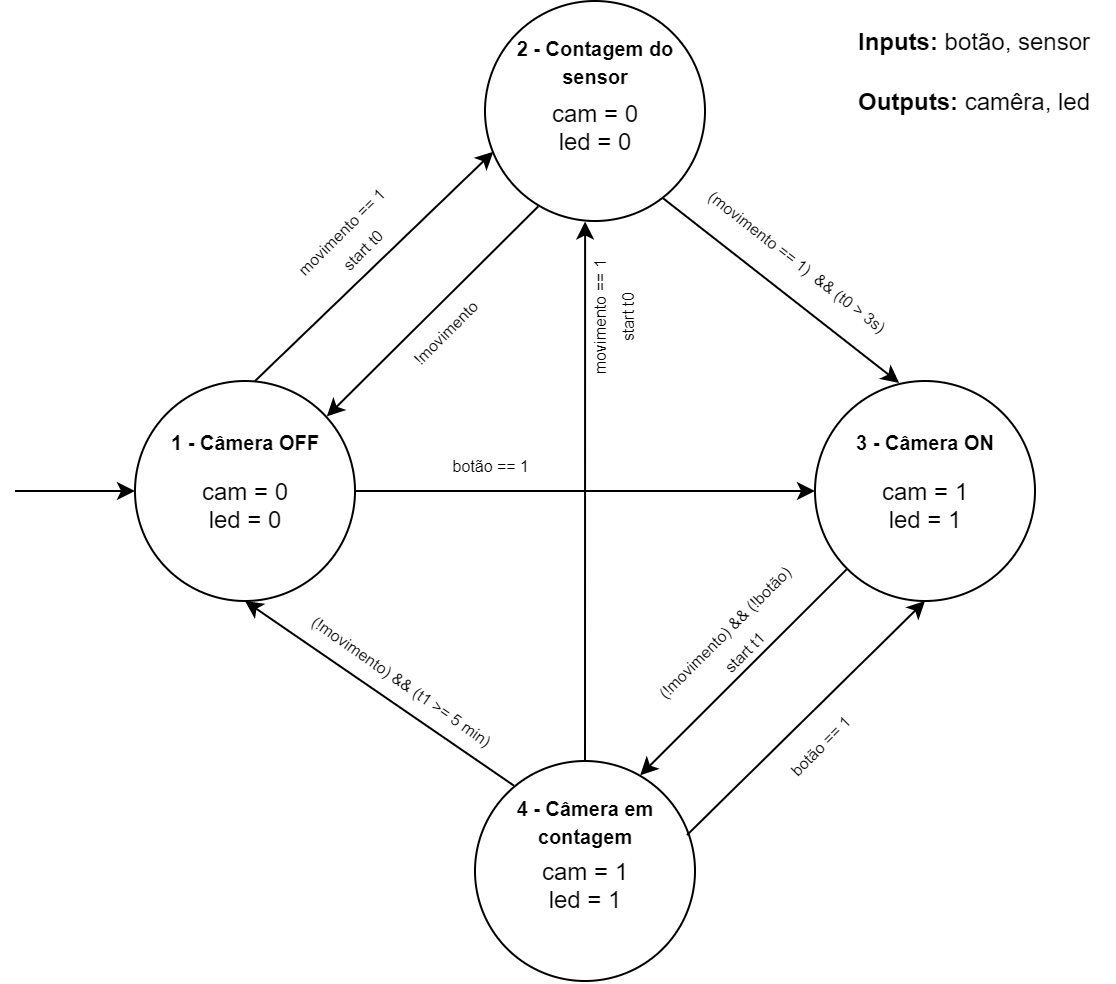
\includegraphics[width=1\textwidth]{diagramas/diagEstado.png}
    \caption{Diagrama de estados}
    \label{fig:diagEstados}
\end{figure}

\begin{itemize}
     \item \textbf{Estado 1}: O ponto de partida ocorre neste estado. Nele, todos os dispositivos encontram-se em \textit{stand by}, sendo assim, o estado \textit{default};
    
    \item \textbf{Estado 2}: Contagem do sensor
        \begin{itemize}
            \item[-] Ocorre após o sensor detetar movimento;
            \item[-] É iniciada uma contagem \textbf{t0}, para verificar se o movimento detetado é intencional. Caso esse movimento seja persistente após 3 segundos, passa-se para o \textbf{estado 3}, caso contrário, volta-se para o estado default;
        \end{itemize}
        
    \item \textbf{Estado 3}: Câmera ON
        \begin{itemize}
            \item[-] A câmera e o led são ligados de duas formas: através do acionamento do botão (proveniente do estado 1), ou pela deteção de movimento intencional (verificado no estado 2).
        \end{itemize}
        
    \item \textbf{Estado 4}: Câmera em contagem \\
    
        \hspace{0.5cm}Após o acionamento da câmera e do led, como foi visto na secção dos \textit{Requisitos},  é necessário estabelecer um tempo máximo em que as mesmas estejam ligadas (5 minutos). Para isso, foram aplicadas as seguintes condições:
        
        \begin{itemize}
            \item[-] Se não for detetado movimento nem acionamento do botão, é iniciada uma contagem \textbf{t1}, em que se o mesmo transpuser os 5 minutos, volta para o \textbf{estado 1}, desligando assim os dois equipamentos;
            \item[-] Durante o intervalo [0,5[ minutos, caso se volte a detetar movimento, é direcionado para o \textbf{estado 2} e caso o botão seja clicado, volta para o \textbf{estado 3}.
        \end{itemize}
    
    
\end{itemize}

\section{Diagrama de hardware/software}

    \begin{figure}[h!]
    \centering
    %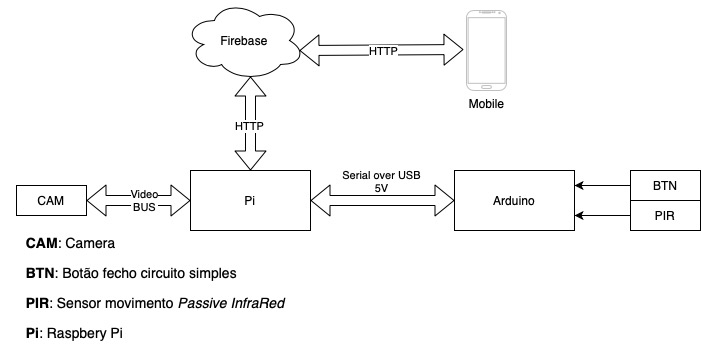
\includegraphics[width=1\textwidth]{diagramas/Diagrama_hardware.jpg}
    \caption{Diagrama de hardware/software}
    \label{fig:diaHardware}
\end{figure}

\begin{itemize}
    \item \textbf{Arduino}: Recebe os estados do botão da campainha e o estado do sensor de movimento. A comunicação destes estados é enviada via serial sobre USB. A escolha do USB ao invés de \textit{RS232} é pelo facto do arduino e o raspberry pi funcionarem com tensões diferentes, sendo necessário um \textit{voltage-shifter}.
    \item \textbf{Raspberry Pi}: Controla a componente da câmera e processa os estados do arduino. Quando é detetado movimento do sensor \textit{PIR} ou do botão ou até receber um pedido via firebase, irá ativar a câmera e começar a capturar fotografias para o cartão SD.
    \item \textbf{Firebase}: Faz a comunicação entre a componente \textit{mobile} e o raspberry pi. Notificações e pedidos são via esta componente.
    \item \textbf{Mobile}: Software client que regista-se no firebase e recebe notificações push. Além das notificações, também tem capacidade de ver o streaming da componente da câmara do raspberry pi.
\end{itemize}

\section{Diagrama de colaboração dos componentes de software}

\begin{figure}[h!]
    \centering
    %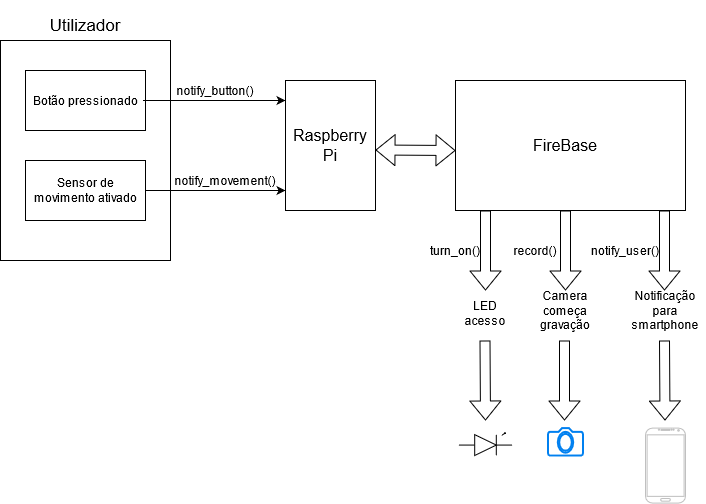
\includegraphics[width=1\textwidth]{diagramas/Untitled Diagram.png}
    \caption{Diagrama de colaboração dos componentes de software}
    \label{fig:diagGantt}
\end{figure}

\begin{itemize}
    \item Neste diagrama, temos representado um utilizador que inicia o todo o processo através de um botão que é pressionado pelo mesmo ou através de movimento que vai ser captado pelo sensor.

    \item Quando estas componentes são ativadas, notificam o Raspberry Pi através das funções notify\_button() e notify\_movement().

    \item O FireBase, que está em permanente conexão com o Raspberry Pi, vai depois accionar as funções para ligar os LED's, que começa a gravação das imagens e que notifica o utilizador no seu smartphone. Estas funções são, respetivamente, turn\_on(), record() e notify\_user().

\end{itemize}

\section{Gantt Chart}

\begin{figure}[h!]
    \centering
    %\includegraphics[width=1.2\textwidth]{diagramas/Gant chart.png}
    \caption{Diagrama de Gantt}
    \label{fig:diagGantt}
\end{figure}




%formulário de requisitos (incluindo custo estimado)
%requisitos funcionais e não funcionais

%Lista:

%- Raspberry Pi Camera Board         9,90 €
%- Sensor de Movimento Mini PIR      4,65 €
%- LED module                        3.00 €
%- Raspberry Pi Camera Board         40.00 €
%- Arduino Uno rev3                  20.00 €
%- 1x Cabo USB                       2.00 €
%- 1x HDMI - Micro HDMI Cable 1.8m   4.00 €
%- 1x  Button 12mm                   1.00 €
%- SD Cards 32 GBs                   5.00 €

% -----------------------------------------------------
% Resumo (Slides ou PDF)
% -----------------------------------------------------~
%
% --------------------
% Objetivos do projeto
% --------------------
% - Implementação de uma câmera e um sensor de movimento na porta de uma casa/apartamento para proporcionar a deteção de presença pessoas.
% - Stream de vídeo a tempo real da entrada da residência no smartphone.
% - Permitir ao utilizador visualizar e apagar vídeos "stop-motion" gravados pela câmera no seu smartphone.
%
%
% ---------------------
% Requisitos Funcionais
% ---------------------
% Captação de imagens "stop-motion" através de uma câmara.
% A câmera ativa quando o sensor deteta movimento ou quando o botão que representa a campainha é clicado.
% Led vermelha indicativa de que a câmera está gravar.
% Passados 5 minutos de deixar de detetar alguém, o sistema deverá parar.
% Utilizador é notificado no smartphone quando alguém toca na campainha
% Utilizador pode requisitar uma stream de video sem "stop-motion" pelo smartphone 
% 

\end{document}
